\begin{appendices}

%Some Table of Contents entry formatting
\addtocontents{toc}{\protect\renewcommand{\protect\cftchappresnum}{\appendixname\space}}
\addtocontents{toc}{\protect\renewcommand{\protect\cftchapnumwidth}{6em}}

%Begin individual appendices, separated as chapters

\chapter{Data} \label{data}
\section{Introduction}
\paragraph{}
During this study we relied for our experiments on a dataset collected and annotated in our team. In this appendix we are going to give more information about this data. From the way we got the base image to distribution of the data on this set, going by the annotation tool we used as the diversity of the case represented.

\section{Data collection}
\paragraph{}
This dataset consist of image of the road taken from the driver perspective with annotations of the visible signs. The data came from two different sources, the first one is image from Nashville DOT, collected by there survey vehicle, equipped with externally mounted high resolution camera. The large majority of the data was, however, collected by our team around Atlanta and in north Georgia. This data collection was done with smartphones and an application specially build for this purpose.

The smartphone used for data collection were of two different model, Xiaomi Redmi 4 and Xiaomi 8. Both of them recorded the video at full HD resolution, at 10 frame per second for the Redmi 4 and 30 frame per second for the Xiaomi 8. Aside from the frame rate, the image quality of this two devices is also completely different. The Redmi 4 produce image that are more blurry and sensitive to over and under exposure, leading to a much lower image quality than Xiaomi 8 that produce much sharper images, although with less natural color that tend to be more blueish.

The Android application we used to collect the data was developed internally and named AllGather. During the data collection the smartphone was attached to the windshield, as displayed on Figure \ref{fig:windshield}. In this setting the smartphone collect the video, as well as the GPS, the acceleration and the value from the magnetometer. Once the the recording the started, it's only needed to drive around the road to collect the data.

\begin{figure}
    \centering
    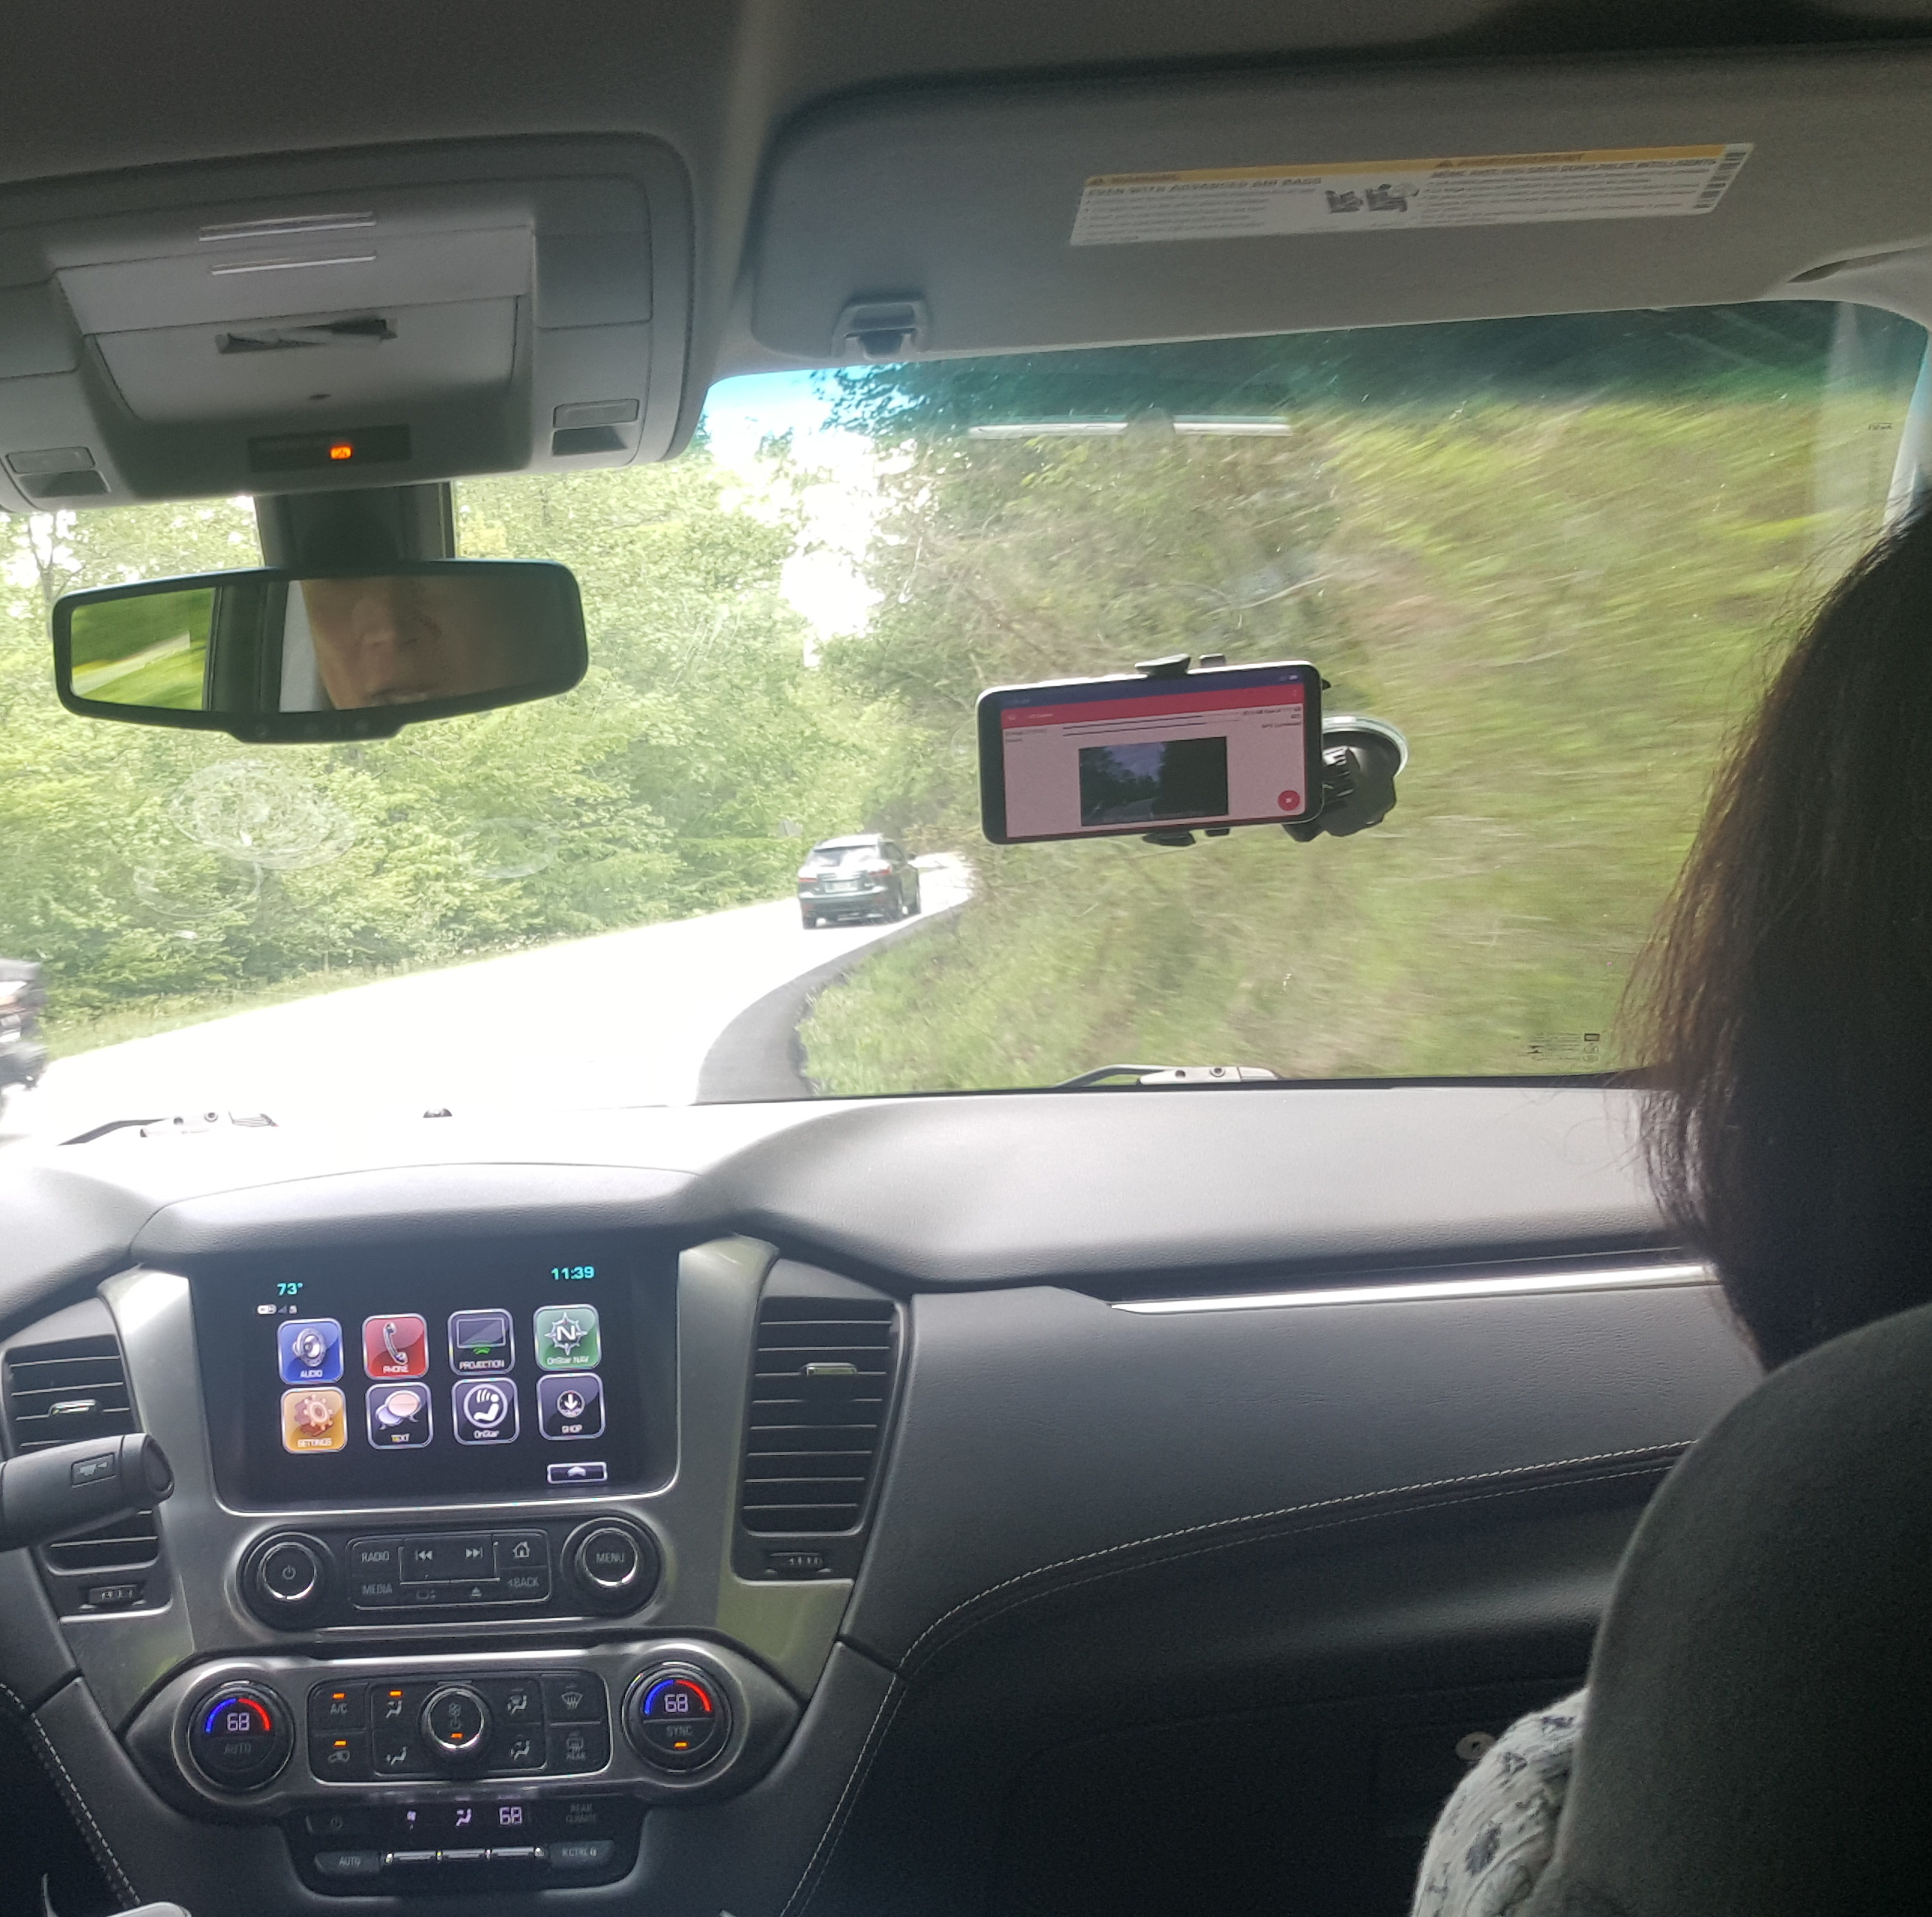
\includegraphics[width=0.5\linewidth]{figures/smartphone-datacolection.jpg}
    \caption{Example of the setup used for data collection}
    \label{fig:windshield}
\end{figure}{}


This process allow to record realistic data real word data, as they are not collected by expensive camera in a especially designed setup. In particular, in addition to the image quality, our image have a fair amount of reflection from the windshield as well as dust. Making this dataset very close to the typical use case.


\section{Data annotation}
\paragraph{}
To perform this study, image alone were not valuable, the more important things is the annotation. To ensure the highest accuracy possible, our team annotated the data internally using a especially made software. 

The software we used for this task is an internal tool developed in C\# to take into account the specificity of our task, especially the video aspect of it. This tool was made to provide more than just the position and class of the signs, it also allow to give id to the signs and signpost or poll. It also implement pattern matching algorithm to make the process of annotating data easier.

This tool was used to annotate all the $652,321$ frames collected, counting $8,719$ sign images spitted in $39$ different classes.

\section{Label distribution}
\paragraph{}
Because our dataset represent the distribution of signs on the local roads of north Georgia. The distribution of the labels in our dataset is quite unbalanced. As you can see on Figure \ref{fig:data_count} and Table \ref{tab:data_count}, some classes of signs are much more represented than other. However, as we only care about detection and not classification, we can group all the warning signs together summing to $8,348$ signs that can be used for training detection. Allowing us to use $8,719$ images during the experiments presented in this document.

\begin{figure}
    \centering
    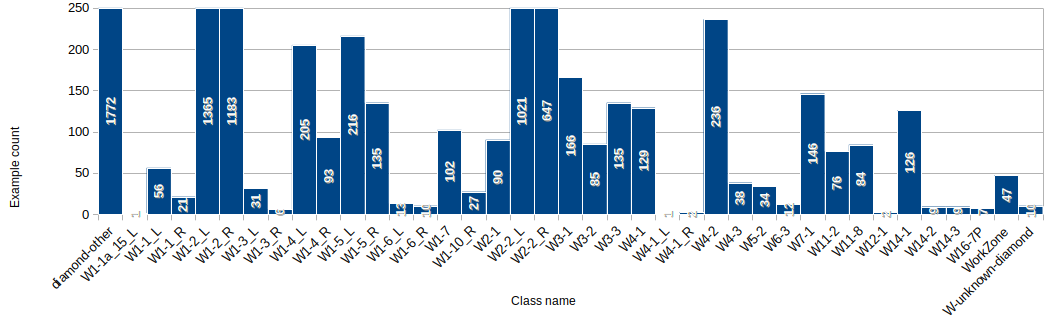
\includegraphics[width=\linewidth]{figures/data_repartition.png}
    \caption{Count of example for each classes in the dataset, cropped to 250 for readability.}
    \label{fig:data_count}
\end{figure}{}

\begin{table}[]
    \centering
    \begin{tabular}{|l|r|}
    \hline
        \textbf{Sign class} & \textbf{Count} \\ \hline
        W1-1a\_15\_L & 1\\
        W1-1\_L & 56\\
        W1-1\_R & 21\\
        W1-2\_L & 1365\\
        W1-2\_R & 1183\\
        W1-3\_L & 31\\
        W1-3\_R & 6\\
        W1-4\_L & 205\\
        W1-4\_R & 93\\
        W1-5\_L & 216\\
        W1-5\_R & 135\\
        W1-6\_L & 13\\
        W1-6\_R & 10\\
        W1-7 & 102\\
        W1-10\_R & 27\\
        W2-1 & 90\\
        W2-2\_L & 1021\\
        W2-2\_R & 647\\
        W3-1 & 166\\
        W3-2 & 85\\
        W3-3 & 135\\
        W4-1 & 129\\
        W4-1\_L & 1\\
        W4-1\_R & 2\\
        W4-2 & 236\\
        W4-3 & 38\\
        W5-2 & 34\\
        W6-3 & 12\\
        W7-1 & 146\\
        W11-2 & 76\\
        W11-8 & 84\\
        W12-1 & 2\\
        W14-1 & 126\\
        W14-2 & 9\\
        W14-3 & 9\\
        W16-7P & 7\\
        WorkZone & 47\\
        W-unknown-diamond & 10\\
        \hline
    \end{tabular}
    \caption{Number of sample for each sign in the dataset}
    \label{tab:data_count}
\end{table}{}

\section{Weather conditions}
Diversity is a key for a machine learning dataset to be successful. By definition, diversity depend on a lot of factor, but in this case one of the important one is the weather. Weather is the main factor defining how far and how clearly you can see objects. Lot of dataset are biased on that point, data are mostly collected in clear sunny day. This dataset is not an exception.

Most of the data where collected while on trip to other fields test. Test that were performed outdoor on pavement and require to avoid rain, ruling out lot of cloudy day in Georgia. However if we don't have bad weather conditions, we our dataset cover still a large set of cases, sunset and darker hours of the day are for example well covered. An illustration of such an image is provided in Figure \ref{fig:blue_hour}.

\begin{figure}
    \centering
    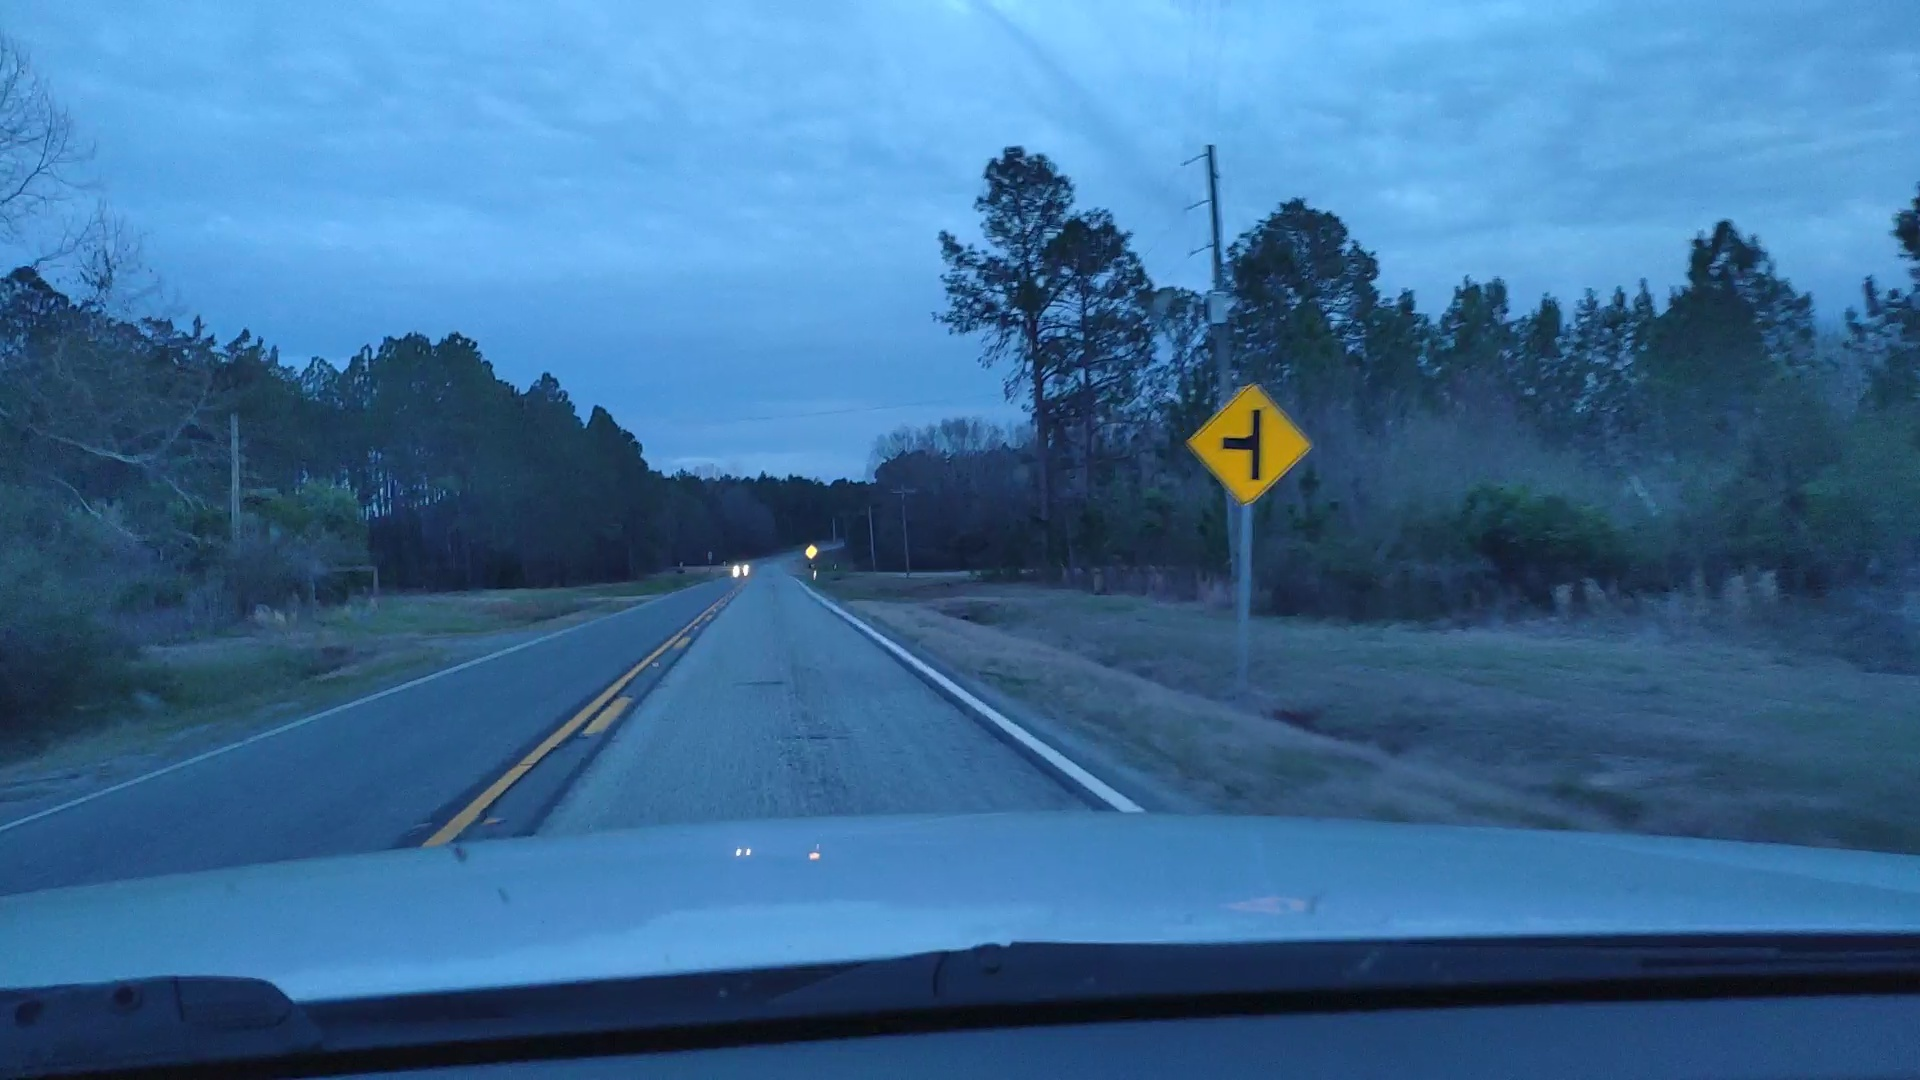
\includegraphics[width=.7\linewidth]{figures/blue_hour_example.jpg}
    \caption{Example of image taken after sunset present in the dataset}
    \label{fig:blue_hour}
\end{figure}{}

This kind of example are very important in the task of traffic sign detection as the appearance of the sign can very a lot under this luminosity condition with the effect of cars lights. this different weather condition also put more importance on the quality of the sign. Newer sign tend to better reflect the light and so are much more visible than old faded one in low light condition, while in plain day light this difference is not that important.

\section{Conclusion}
\paragraph{}
This dataset collected and annotated manually by our team, is a corner stone of this project. This dataset has it's own issue and could be improved, some weather conditions are missing, classes are largely unbalanced and the number of image is fairly limited. However, for our task of object detection on small scale models, such imperfection are not really critical.


\end{appendices}